\newcounter{nuserstory}
\newcounter{nusecase}

\newcommand{\userstory}[4]{%
    \refstepcounter{nuserstory}
    \subsection{#1}
    \label{userstory:\thenuserstory}
    \hangindent=40pt
    \textbf{\textit{As a}} #2,\\
    \textbf{\textit{I want to}} #3,\\
    \textbf{\textit{so that}} #4.
}
\newenvironment{usecase}[1]
{
    \refstepcounter{nusecase}%
    \subsection{Use Case \thenusecase: #1}%
    \label{usecase:\thenusecase}%
}{}

% With user stories (\userstory) you can reference them back later with \ref{userstory:n}
% For example, first user story in this file can be referred with \ref{userstory:1}

\chapter{Requirement Analysis}
\label{chap:requirement-analysis}

\section{Stakeholder Analysis}
\label{section:stakeholder-analysis}

\subsection{Primary Stakeholders}
\label{subsection:primary-stakeholders}

\begin{enumerate}[leftmargin=80pt]
    \item \textbf{Users:} The primary stakeholders are users of our application,
    they have a key role to populate our application's data, and evaluate our project's impact.
    For specification of our users see \ref{section:target-user}.
    \item \textbf{Food stall owners:} Owners of food stalls in cafeterias on Kasetsart University grounds
    is our primary source of data acquisition. With KU Eater, we make sure to bring positive changes not just to
    consumers but also the producers.
\end{enumerate}

\section{User Stories}
\label{section:user-stories}

%% User Stories Start

\userstory{Menu Items at Fingertips%
}{user of cafeteria in Kasetsart University%
}{know what menus are available in the stalls beforehand%
}{I don't need to waste my time choosing at the cafeteria}

\userstory{Recommending Trending Food Items%
}{user of cafeteria in Kasetsart University%
}{be able to see what kinds of dish are trending by other students%
}{I will have best food choices to try out}

\userstory{Recommending Food Items based on Dietary Restrictions%
}{user of cafeteria in Kasetsart University with a dietary restriction%
}{be able to see what kinds of dish are offered for people with same dietary restriction%
}{I get to know what are the best food items I can have at the cafeteria}

\userstory{Searching Food Items with Specific Names%
}{user of cafeteria in Kasetsart University%
}{be able to search for a specific dish%
}{I can pinpoint where to get a food item that I want}

\userstory{Filtering Food Items based on Dietary Restrictions%
}{user of cafeteria in Kasetsart University with a dietary restriction%
}{search and filter for menu items that satisfies my dietary restriction%
}{I get my own list of dishes that I can have to browse}

\userstory{Reviewing Menu Items Offered%
}{customer of a food stall in a cafeteria of KU%
}{post a review of the food item I get at the stall%
}{other users can read my review and know more about food offered at the stall}

\userstory{Comparing Similiar Dishes of Different Stalls%
}{certain food lover who dines at a cafeteria in KU%
}{see differences of reviews that of the same food item but offered by different stalls%
}{I get to compare and choose to purchase the specific dish between the stalls}

%% User Stories End

\section{Use Case Diagram}
\label{section:use-case-diagram}

\begin{figure}[h!]
    \centering
    \begin{tikzpicture}

        \begin{umlsystem}[x=4]{KU Eater}
            \umlusecase[name=signup, y=4.5]{Sign Up}
            \umlusecase[name=login, y=3]{Login}
            \umlusecase[name=viewrec, y=1, width=2.5cm]{View Recommendations}
            \umlusecase[name=genrec, x=6.5, y=2, width=2.5cm]{Generate Recommendations}
            \umlusecase[name=menuinfo, x=4, y=0.25]{See Menu Info}
            \umlusecase[name=searchmenu, x=1, y=-1]{Search Menu Items}
            \umlusecase[name=userrec, x=6.5, y=-4, width=3.5cm]{Personalized Recommendations}
            \umlusecase[name=trendrec, x=6.5, y=4.5, width=2.5cm]{Trending Recommendations}
            \umlusecase[name=readreview, y=-2.5]{Read Reviews}
            \umlusecase[name=writereview, x=-0.25, y=-4]{Write Review}
            \umlusecase[name=rateitem, x=1, y=-5.5]{Rate Menu Items}
            \umlusecase[name=editprofile, x=3, y=-7]{Edit Profile}
        \end{umlsystem}

        \umlactor[y=-1]{User}
        \umlactor[y=3]{Guest}
        \umlactor[y=-5]{Member}
        \umlactor[x=15]{System}

        \umlassoc{Guest}{login}
        \umlassoc{Guest}{signup}
        \umlassoc{User}{viewrec}
        \umlassoc{User}{menuinfo}
        \umlassoc{User}{searchmenu}
        \umlassoc{User}{readreview}
        \umlassoc{Member}{writereview}
        \umlassoc{Member}{rateitem}
        \umlassoc{Member}{editprofile}
        \umlassoc{System}{genrec}
        \umlinclude{viewrec}{genrec}
        \umlinclude{userrec}{writereview}
        \umlinclude{userrec}{rateitem}
        \umlinclude{userrec}{editprofile}
        \umlinherit{Guest}{User}
        \umlinherit{Member}{User}
        \umlinherit{userrec}{genrec}
        \umlinherit{trendrec}{genrec}

    \end{tikzpicture}
    \caption{Use Case Diagram of KU Eater}
    \vspace*{-1in}
\end{figure}

\section{Use Case Model}
\label{section:use-case-model}

% Use Cases Start

\begin{usecase}{Viewing the Menu}
    \textbf{Actors:} Tom (Cafeteria User), KU Eater (System)
    
    \textbf{Description:} Tom wants to see the food items being offered at the cafeteria.

    \textbf{Scenario:}

    \begin{enumerate}[leftmargin=80pt]
        \item Tom opens KU Eater application on his device.
        \item System renders the main page which contains recommendations and browsable list of menus and stalls.
        \item Tom can now browse the menu of each stalls and choose his favorite food.
    \end{enumerate}
\end{usecase}

\begin{usecase}{Seeing Recommendations on Trending Menu}
    \textbf{Actors:} Tom (Cafeteria User), KU Eater (System)
    
    \textbf{Description:} Tom doesn't know what to eat, so he wants to find any stalls that could be good. The metrics
    for good food is popularity.

    \textbf{Scenario:}

    \begin{enumerate}[leftmargin=80pt]
        \item Tom opens KU Eater application on his device.
        \item System starts to generate lists of recommendations, one of the list "Now Trending" scores the recommendations
        based on average user ratings and review scores.
        \item System renders back to Tom with an amount of topmost trending stalls and their menus.
        \item Tom clicks on "See More."
        \item System renders a scrollable list of more trending stalls.
        \item Tom can now browse a list of menu items which are trending.
    \end{enumerate}
\end{usecase}

\begin{usecase}{Seeing Personalized Recommendations}
    \textbf{Actors:} Amber (Cafeteria User), KU Eater (System)
    
    \textbf{Description:} Amber has been using KU Eater for a while and is now a member, she's has a pattern of liking seafood.
    She wants to discover food choices available in the app.

    \textbf{Preconditions:} Amber is a member and has rated and loved seafood in the cafeteria.

    \textbf{Scenario:}

    \begin{enumerate}[leftmargin=80pt]
        \item Amber opens KU Eater application on her device.
        \item System starts to generate lists of recommendations, one of the list "For You" scores recommendations
        based on similiarity of user preferences and menu database.
        \item System renders back to Amber with an amount of relevant stalls and their menus.
        \item Amber clicks on "See More."
        \item System renders a scrollable list of more suitable stalls.
        \item Amber can now browse a list of menu items which are mostly seafood and tailored for her.
    \end{enumerate}
\end{usecase}

\begin{usecase}{Searching for a Specific Dish}
    \textbf{Actors:} John (Cafeteria User), KU Eater (System)
    
    \textbf{Description:} John wants to have boat noodles for lunch. He's using KU Eater to speed up
    his process of finding.

    \textbf{Scenario:}

    \begin{enumerate}[leftmargin=80pt]
        \item John opens KU Eater application on his device.
        \item System renders the main page with search bar at the top.
        \item John clicks on Search bar and types in "boat noodles."
        \item System looks for stalls that sells boat noodles and renders a collective list of relevant stalls.
        \item John will now see many stalls selling boat noodles.
    \end{enumerate}
\end{usecase}

\begin{usecase}{Filtering with Dietary Restrictions}
    \textbf{Actors:} Harry (Cafeteria User), KU Eater (System)

    \textbf{Description:} Harry is allergic to bell peppers, however he wants to have stir-fry which some stalls cook with bell peppers.
    He wants to find stalls that serve his way.

    \textbf{Scenario:}

    \begin{enumerate}[leftmargin=80pt]
        \item Harry opens KU Eater application on his device.
        \item System renders the main page with search bar at the top.
        \item Harry clicks on Search bar and types in "stir-fry."
        \item Harry also puts in filter as he doesn't want to include "bell peppers."
        \item System looks for stalls that sells stir-fry with no bell peppers and renders a collective list of relevant stalls.
        \item Harry will be able to browse the many relevant stalls.
    \end{enumerate}
\end{usecase}

\begin{usecase}{Reading Reviews on Specific Stall}
    \textbf{Actors:} Tom (Cafeteria User), KU Eater (System)

    \textbf{Description:} Tom founds a trending dish on three stalls, however he wants to compare between each stalls.

    \textbf{Scenario:}

    \begin{enumerate}[leftmargin=80pt]
        \item Tom opens KU Eater application on his device.
        \item System renders the main page which contains recommendations and browsable list of menus and stalls.
        \item Tom sees three stalls that sell fried chicken---which piques his interest.
        \item Tom clicks on one of the stalls.
        \item System retreives the most relevant reviews which are for fried chicken and renders them as a list.
        \item Tom can now read the reviews on a specific stall.
    \end{enumerate}
\end{usecase}

\begin{usecase}{Writing Review for a Dish in Stall}
    \textbf{Actors:} Mike (Cafeteria User), KU Eater (System)

    \textbf{Description:} Mike has just finished his meal and would like to get his thoughts on the dish to the platform.

    \textbf{Preconditions:} Mike is a member on KU Eater.

    \textbf{Scenario:}

    \begin{enumerate}[leftmargin=80pt]
        \item Mike opens KU Eater application on his device.
        \item System renders the main page.
        \item Mike goes to the correct stall page and clicks on his eaten menu item.
        \item System renders information about his meal, including ingredients and other reviews.
        \item Mike clicks on "Add Review," and writes his thoughts before hitting submit.
        \item System redirects Mike back to the same menu item page with his comment now added.
    \end{enumerate}
\end{usecase}

\begin{usecase}{Rating a Dish in Stall}
    \textbf{Actors:} Carol (Cafeteria User), KU Eater (System)

    \textbf{Description:} Carol has just finished her meal and wanted to help the stall gain more traction, but is lazy to be writing reviews.

    \textbf{Preconditions:} Carol is a member on KU Eater.

    \textbf{Scenario:}

    \begin{enumerate}[leftmargin=80pt]
        \item Carol opens KU Eater application on her device.
        \item System renders the main page.
        \item Carol goes to the correct stall page and finds her menu item.
        \item Carol clicks on "Thumbs Up" button.
        \item System records her rating and uses it to re-rank the stalls.
    \end{enumerate}
\end{usecase}

% Use Cases End

\section{User Interface Design}
\label{section:user-interface-design}

\begin{figure}[h!]
    \centering
    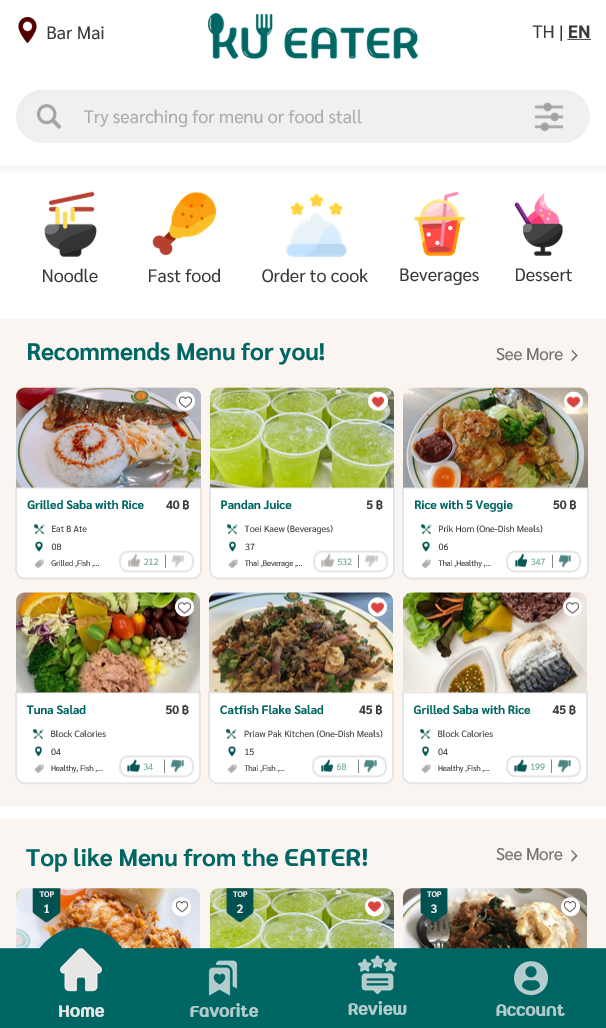
\includegraphics[height=5in]{kueater/homepage.png}
    \caption{Mockup of Homepage}
    \vspace*{-\baselineskip}
\end{figure}